\clearpage
\section{Arduino Quantum Receiver}

\begin{refsection}
	
	\begin{tcolorbox}	
		\begin{tabular}{p{2.75cm} p{0.2cm} p{10.5cm}} 	
			\textbf{Student Name}  		&:&  Jo\~ao Fraz\~ao (2019/09/02 - )\\
			&:&  Eduardo Fernandes (2019/06/15 - 2019/09/14)\\
			\textbf{Goal}          &:& Implement the QKD reception module in an Arduino (Coincidence Detector, QBER, Source and Sink blocks).\\
			\textbf{Directory}              &:& sdf/arduino\_quantum\_rx
		\end{tabular}
	\end{tcolorbox}
 
    \subsection{Introduction }
    In order to have a quantum cryptography system working, we need to have a safe environment in which Alice and Bob do their communications. This two entities represent the transmitter and the receptor side, and are connected by a quantum channel. On one hand, Alice encodes her random bits in the polarization state of the single photons using two sets of non orthogonal bases. This means that, she can manipulate four states of polarization to encode her  photons. For each transmission, Alice encodes her bit in a randomly polarization state and sends it throught the quantum channel to Bob. This channel corresponds to the optical fiber that connects the two entities. Here is where Eve can gain access, and tries to steal information from the system. However, when she does a measurement, she destroys the photon and cannot replicate it. On the other hand, Bob without knowing Alice's basis selection, randomly measures the photon in one of the two non orthogonal bases. If they chose the same one, they can generate correlated random bits. However, if they used different bases, their bit values are uncorrelated and this information is discarded. Alice and Bob, communicate via classic channel and compare the two sequences that identifies the bases used in preparation of the initial states, and the ones used to measure the final states.

	\subsection{Project definition }
	For the receiver side of the QKD implementation, it was needed a soltution that could compensate the random polarizations rotations from the optical fibers (quantum channel), and that could do the commutations of the bases according the QBER reports in real time. The basic idea, is to one arduino reading the output signal of the single photon detectors when they click and to the coincidence check. This coincidence block in the arduino is going to send the integer 3 if non of the detectors clicked, 2 if both clicked, 1 ir 0 depending if one measured photon and the other did not. This information is sent to a computer through a USB connection. Here we have a program receiving the data and sending it via a TCP/IP connection to the QBER block in the Netxpto. This program is going to calculate the QBER every clock cycle outputting a report file with the respect results. According to this results a second arduino is going to adjust an external DAC, in order to manipulate the eletronic polarization controllers to compensate the polarization and change the bases.

	
		\begin{figure}[H] 
		\centering
		\includegraphics[width=1\linewidth]{./sdf/arduino_quantum_rx/figures/diagrama33.pdf}
		\caption{Block diagram of a arduino implementation.}
		\label{fig:netxpto}
		
	\end{figure}
	In figure 5.1, it is represented the final architecture  of the reception modules using Arduinos, after all the trials and tests that were done in the laboratory.
	
	\subsection{Technology equipment}
	Before explaning in detail all the processes of the proposed arquitechture, we need to have a general view of the individual equipments used in the implementation:
	
		
		\subsection{Detectors}
		The photon counting is done by two ID Quantique's single photon detectors module. The core consists of a InGAaS/InP avalanche photodiode. In order to reduce the dark count probability, the APD is cooled using a thermoeletric cooler. The APD is operated in the gated mode, where a voltage pulse is applied to raise the bias beyond the breakdown point. This type of techonology allows a single photon sensivity ip to a wavelenght of 1650 nm. The performance of an APD is characterized by the probability for a photon impinging on the photodiode to be detected. At 1550 nm, which is the wavelenght we are using in laser on the transmitter side, a 25\% detection efficiency is typical. In the APD, avalanches can also be triggered by carriers generated in thernam, tunneling or trapping processes taking place in the junction. These  self-triggering effects are called dark counts, and reresents the probability as a function of the detection efficency at a temperature of 220 K. At 10\% detection efficiency, the dark count probability is typically  $6* 10^{-5} ns^{-1}$ or less. The main problem limiting the performance are the afterpulses. This spurious effect arises from trapping of  charge carriers during an avalanche by trap levels inside the high field region of the junction where impact ionization occurs.
		
		\begin{figure}[H]
			\centering
			\includegraphics[width=0.8\linewidth]{./sdf/arduino_quantum_rx/figures/detectors.PNG}
			\caption{Single photon detectors}
			\label{fig:arduino}
		\end{figure}
		
		
		
		\subsection{Clock divider board}
		This custom made board simply, takes the signal coming from the classic detector and divides it to the two single photon detectors and the arduino. This signal represents the clock and is going to keep the system synchronized.
		
	
	    \subsection{Arduino DUE}
	     Arduino represents an open-source platform that consists of both a physical programmable circuit board, containing a microcontroller, and an  Integrated Development Enviroment that runs is a computer through an USB cable.
	    The Arduino model used for this project was the DUE. It has a microcontroller board based on the Atmel SAM3X8E ARM Cortex-M3 CPU. It also has 54 input/output pins, 12 analog inputs, 4 UARTs, 84 MHz clock, 2 DAC, 2 TWI, a power jack, an SPI header, JTAG header, a reset button and an erase button. However this model is limited at 3.3V for the maximum voltage that the I/O pins can tolerate.  
	    
	    \begin{figure}[H]
	    	\centering
	    	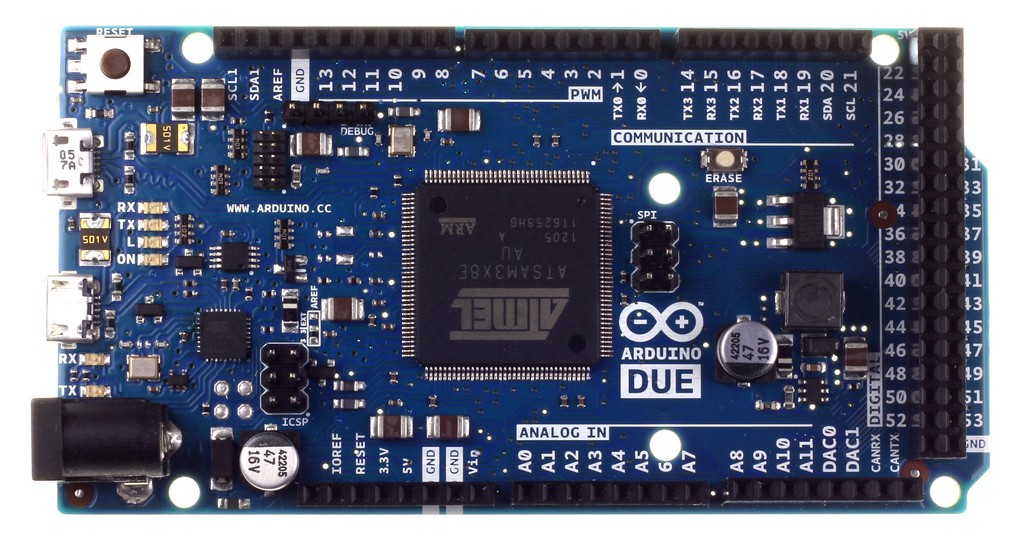
\includegraphics[width=0.8\linewidth]{./sdf/arduino_quantum_rx/figures/arduino.PNG}
	    	\caption{Arduino Due.}
	    	\label{fig:arduino}
	    \end{figure}
	    	
	    In order to utilize the same project running over NETXPTO simulator using Arduino technology some changes in the source code had to be made once this technology uses C/C++ language features while relying on special rules of code structuring. Acoording to Arduino official manufactures this language is merely a set of C/C++ functions that can be called from your code. Your sketch undergoes minor changes (e.g. automatic generation of function prototypes) and then is passed directly to a C/C++ compiler (avr-g++).However, there's currently no support for libstdc++, the standard support library needed for a complete C++ implementation. This imposes a number of restrictions on the C++ programs that can be compiled. Among them are:
	    
	    \begin{itemize}
	    	\item Some of the C++ related standard functions, classes, and template classes are available.
	    	\item The operators new and delete are not implemented, attempting to use them will cause the linker to complain about undefined external references.
	    	\item Some of the supplied include files are not C++ safe.
	    	\item Exceptions are not supported.
	    	\item When programming C++ in microcontrollers, extra care should be taken to avoid unwanted side effects of the C++ calling conventions like implied copy constructors that could be called upon function invocation etc.
	    	\item The outputs to the console have to be made through the arduino serial monitor using the function Serial.print() instead of making use of cout, cin or cerr classes.
	    	\item  The implementation of a non-specialized template methods must be visible to a translation unit that uses it. The compiler must be able to see the implementation in order to generate code for all specializations in your code. This can be achieved in two ways: either by moving the implementation, the cpp file, inside the header or if you want to keep it separate, move it into a different header which you include in your original header.
	    	\item Arduino does not recognize objects of type std::initializer\_list<T>, which are a lightweight proxy object that provides access to an array of objects of type const T, so instead we have to use vector containers in order to initialize the constructors attributes.
	\end{itemize}

	\subsection{AD5669 DAC}
	The AD5669 is a I2C high-resolution digital to analog converter capble of generating a 0-5V voltage output. It has a 16-Bit resolution and is capble of tuning the output across 65,536 setps. It is equiped with 8 individual output channels and one floating adress line. The AD5669 is capable of 400 kHz communication speed , making it ideal for programmable voltage and current source applications. It is compatible with the Arduino by including the Wire.h library and defining the DAC adress in the program.
	In the arduino program we set the correct adress of the AD5669. It also requires two bytes of data for the DAC and a command byte that controls all the various functions. The clock chose was 400 kHz, to achieve maximum speed, and four channels were set to output random voltages. Using the Wire library functions, the I2C transmission is established in order to control all four channels accordingly.
	
		\begin{figure}[H]
		
		\centering
		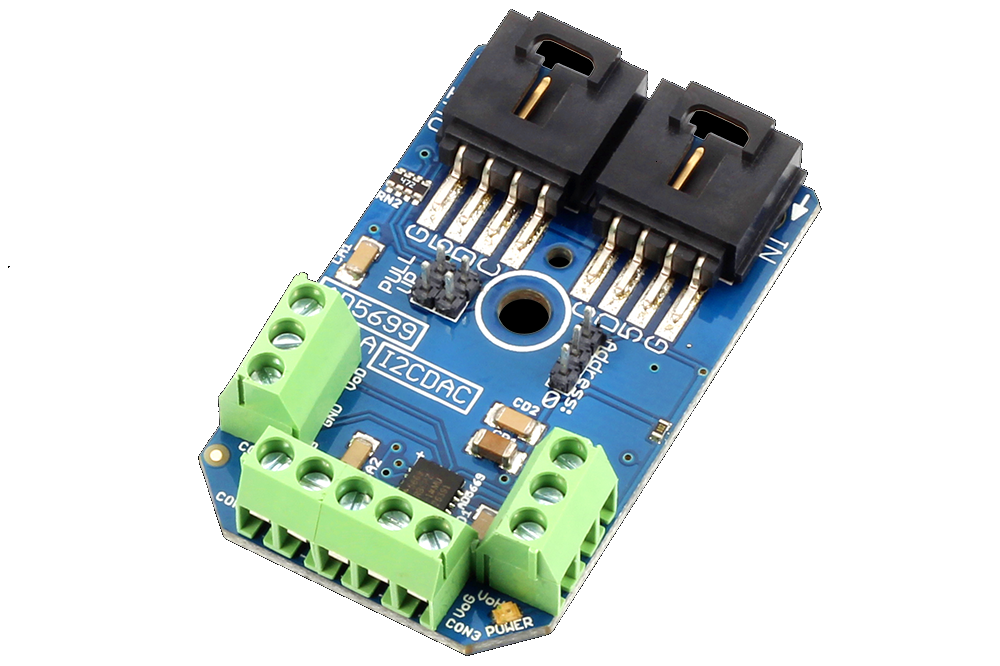
\includegraphics[width=0.6\linewidth]{./sdf/arduino_quantum_rx/figures/dac2.png}
		\caption{AD5669 DAC}
		\label{fig:netxpto}
		
	\end{figure}

	\subsection{Polarization controller}
	Polarization controllers can be operated without feedback, typically by manual or electrical adjustments or wiht an automatic feedback. A polarization controller can transform a fixed, known polarization into an arbritary one. In the reception side, these are used to compensate the random polarization drift from the quantum channel and used to choose in which base the single photons are going to be measured. The ones used in the laboratory need four voltage inputs in order to operate. Since these ones are electro-mechanical, we may get different results when the same voltages are applied in different occasions. 
	
	
	\subsection{Arduino implementation - Signal acquisition}
	As mention before, we have one Arduino reading the signals of the quantum detectors each clock cycle and sending this data to a computer. For the signal acquisition we had two options: polling mode or the interruption mode. Polling proved impossible to implement, since the quantum detectors output signal had a maximum width of 100 ns,in contrast to the minimum time of 523 ns for the digitalRead() function to be completed. This means we cannot read two signals simultaneously, and would always be loosing information each cycle. The right approach is to use an interruption every time rising edge coming from the single photon detectors or the clock signal is caught. To do this, all the receiving signals are read in the digital input pins of the Arduino DUE board. This type of reading doesn't require any signal conditioning, which means we can take measures directly into the Arduino. Since we can control all the voltages, we just need to be careful to not set them above the 3.3V max input threshold of the Arduino DUE. The clock trigger reaches the detectors and the Arduino at the same time. In order to detect it, the Arduino does an interruption when it catches a rising voltage and puts a Boolean to true, meaning it is ready to take the output signal from the detectors.
	Since it is also possible to control the TTL signal voltage that comes from the single photon detectors gate, we can measure them directly into the Arduino board through the digital input pins. When the clock reaches the detectors, they send a pulse through the gate into the DUE board. The Arduino does an interrupt function in order to catch the rising edge and puts a Boolean to true. If the Arduino has the two booleans
	of the detectors true, it will print to the serial COM a 2. If none of the detectors clicked, only the clock boolean is true and it is going to print a 3. Depending on if one detector clicked and the other did not, one Boolean is going to be true and the other false, and the Arduino is going to print a 0 or 1.
		
	\subsection{Arduino implementation- Communication with Netxpto}
		
	To have the set up running we need to open three different programs in the arduino\_real\_time\_receiver paste and run them at the same time: ardRece.ino, serial\_port\_reader\_writer.sln (client side) and netxpto\_qber\_estimation.sln (server side).
	The Arduino program has the 26,27 and 28 pins in the INPUT mode, waiting for an external signal from the clock or the detectors. Each one of the pins, is attached to an interruption that takes place when a rising edge is caught. When an interruption is triggered, the program does a function that puts a boolean to true. There is four possible results that are going to be printed in the COM port.
	Even though, the attachInterrupt function takes about 2 microseconds to be done, this does not represent a problem, because the arduino saves the register of another event during an interruption.
	Every external clock cycle, the program does one print a resets all the booleans to false.
		
	Afterwards the Arduino outputs the values of the coincidence block, we need to send the data to a PC, in order to do the calculation of the QBER in real time. To have this implemented in our system, we have the Arduino sending the data one by one to a c++ program in the PC via USB cable. The serial\_port\_reader\_writer.sln program (client side), waits for a connection with the Arduino Serial port in order to start receiving the data. Now that the communication between the Arduino serial port and the PC is done, the program burns the first 10 seconds of information because the Arduino tends to send unnecessary bits when it starts writing in the COM. The program puts the receiving information in a buffer and when it's full, all the data is sent to the QBER program. This means we have a TCP/IP connection between the program reading the Arduino data and the one that does the QBER estimations. The size of the buffer is 4000 characters. In order to always have the correct values of the QBER we need to have the sequence the Arduino is sending synchronized with the sequence from the Alice side. To do this, we have the QBER program running in two modes, the synchronized one, and the unsynchronized. After burning the unnecessary data, it is going to check the first few bits in the buffer and compare it with the transmitter sequence. If they are different, the program will discard the first bit that entered the sequence and add a new one (FIFO). This occurs until we have a match in the sequences, and the program will run normally in the synchronized mode. If, for some reason, the program loses the synchronization, it will do the same process previously explained. In the two modes the program will always output a file, the midreports, every 8000 bits, with the results of the QBER block calculations. 
		
		\begin{figure}[H]
			\centering
			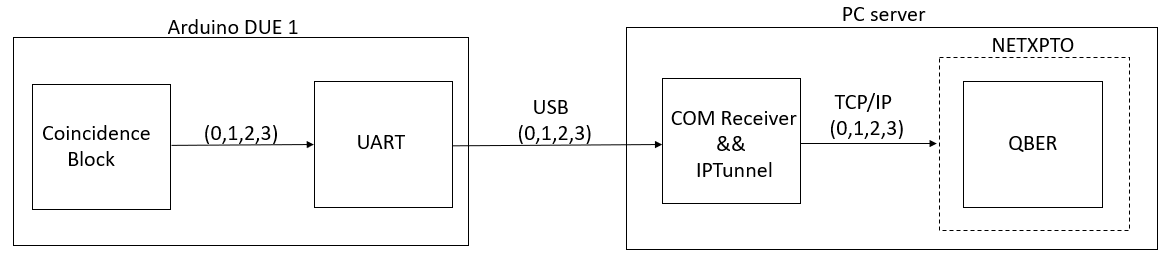
\includegraphics[width=1\linewidth]{./sdf/arduino_quantum_rx/figures/PC.png}
			\caption{Block diagram of Arduino to NETXPTO communication.}
			\label{fig:netxpto}
		\end{figure}
	
	
	\subsubsection{Arduino Implementation - Electronic Polarization Controller }
	In this implementation we also need to control in which base Bob is receiving the data. This set up is going to be able to change between two different basis, so that Bob can choose the base to measure the single photons coming from Alice. To have the basis changing, we have to apply four voltages to an EPC. However, the Arduino only has two internal DACs and needs to receive data from NETXPTO. For the first problem, we are using an AD5669 external DAC, that is communicating with the Arduino via I2C protocol that can output 8 signals. Also, the Arduino can't be receiving and sending data through the same serial COM because it will lose synchronization, therefore loosing bits over time. That is the reason we are using two Arduinos: One takes the clock, the output signals, and sends them to a PC via USB. The other one is just receiving information from the NETXPTO program, and setting the correct voltages to a DAC. The two Arduinos are syncrhonized by the external clock trigger. However, the process of sending data through the PC to the serial COM  is limited by the PC performance. This means at certain frequencies of the clock, the PC might be doing a lot of operations internally affecting the synchronization. The limit of the speed is around 2.5 kHz, which does not represent a problem right now since the system, in a first stage, will be working at 500 Hz. The Arduinos need to do all these operations while the detectors are waiting for the next clock pulse. 
	
	
	\begin{figure}[H]
		
		\centering
		\includegraphics[width=1\linewidth]{./sdf/arduino_quantum_rx/figures/DAC.png}
		\caption{Block diagram of NETXPTO to EPC communication.}
		\label{fig:netxpto}
		
	\end{figure}
	
	Even though we are using two Arduinos, we just do some modifications in the Arduino program previously presented. Since the implementation uses an external DAC, the Arduino needs to communicate with it using a I2C protocol. To do that we need to include the wire library, and use its functions to begin the communication, set the clock speed, write the voltage data to the DAC output and to end the transmission.
	
	\subsubsection{QBER Results }
	

   \clearpage
	
	\subsection{Visual Studio 2019 - Installation guide (Current version: 16.2.3)}
	
	\subsubsection{Step 1}
	
	The first thing to do is to download the bootstrapper file of this software through the following link: https://visualstudio.microsoft.com/pt-br/downloads/. As seen below in figure \ref{vstudio} one of three available versions can be choosen.
	
	\begin{figure}[H]
		\centering
		\includegraphics[width=1\linewidth]{./sdf/arduino_quantum_rx/figures/vsDownload.pdf}
		\caption{Download page of Visual Studio IDE software.}
		\label{vstudio}
	\end{figure}
	
	
	\subsubsection{Step 2}
	
	Execute the installer file, which you can use to customize your installation by selecting the feature sets or workloads, individual components, language packs and installation locations, as demonstrated in figure \ref{vstudioWorkloads}.
	
	
	
	\subsubsection{Step 3}
	
	The installation is quite simple and contains few steps for its execution, in case there is any doubt or question you can always get support from https://docs.microsoft.com/en-us/visualstudio/install/install-visual-studio?view=vs-2019.
	
	\begin{figure}[H]
		\centering
		\includegraphics[width=1\linewidth]{./sdf/arduino_quantum_rx/figures/VSworkloads.pdf}
		\caption{Modifying - Visual Studio 2019.}
		\label{vstudioWorkloads}
	\end{figure}
	
	\subsection{Arduino IDE - Installation guide (Current version: 1.8.9) for Windows machines}
	
	\subsubsection{Step 1}
	
	Download the latest version of Arduino desktop IDE installer file from https://www.arduino.cc/en/main/software.
	
	\begin{figure}[H]
		\centering
		\includegraphics[width=0.86\linewidth]{./sdf/arduino_quantum_rx/figures/arduinoDownload.pdf}
		\caption{Download Arduino IDE software.}
		\label{arduinoDownload}
	\end{figure}
	
	
	\subsubsection{Step 2}
	
	When the download finishes, proceed with the installation and allow the driver installation process when you get a warning from the operating system. Follow the help guide present in https://www.arduino.cc/en/Guide/Windows.
	
	\subsubsection{Step 3}
	
	Proceed with the board specific instructions by going to https://www.arduino.cc/en/Guide/HomePage and selecting the respective board from the list provided, for this specific case we are considering the Arduino Due and so you can use the following link: https://www.arduino.cc/en/Guide/ArduinoDue.
	
	\begin{figure}[H]
		\centering
		\includegraphics[width=1\linewidth]{./sdf/arduino_quantum_rx/figures/arduinoBoards.pdf}
		\caption{Select instructions for you specific board, in this case, the Arduino Due.}
		\label{arduinoDownload}
	\end{figure}
	
	\subsection{Visual Micro - Installation and Setup guide}
	Visual Micro is a plugin for Microsoft Visual Studio that helps you creating Arduino compatible cross-platform programs for hundreds of different Arduino compatible micro-controllers. Visual Micro supports projects that contain one or more .ino code files and standard c++ cource code files, just like the Arduino IDE.
	
	
	\subsubsection{Step 1}
	Download Visual Micro from here https://www.visualmicro.com/page/Arduino-Visual-Studio-Downloads.aspx or it can also be installed and uninstalled from inside the IDE, by opening Visual Studio and clicking "Extensions>Manage Extensions>Online>Arduino IDE for Visual Studio".
	
	\subsubsection{Step 2}
	If Visual Studio/Atmel Studio is running, then close it.
	
	\subsubsection{Step 3}
	Install Visual Micro by doubleclicking on the "vsix" icon of the downloaded file or in the case you are installing it from within the Visual Studio IDE it will start automatically.
	
	\subsubsection{Step 4}
	
	The first time, after you have installed Arduino for Visual Micro, the Configuration Manager will pop up where you can configure your system. Visual Micro must know the version and installation path of the Arduino IDE software that you have installed in your computer.
	
	\begin{figure}[H]
		\centering
		\includegraphics[width=1\linewidth]{./sdf/arduino_quantum_rx/figures/configureIDE.pdf}
		\caption{Configure IDE locations.}
		\label{configureIDE}
	\end{figure}
	
	\subsubsection{Step 4}
	If you work with different boards that required different IDEs, or if you have multiple versions of the Arduino IDE installed, then repeat the steps above for each IDE. It is possible to switch between configurations with the toolbar presented below in figure \ref{}.
	
	\begin{figure}[H]
		\centering
		\includegraphics[width=0.7\linewidth]{./sdf/arduino_quantum_rx/figures/multipleIDEversions.pdf}
		\caption{Support for Multiple Versions of the Arduino Softwares.}
		\label{multipleIDEversions}
	\end{figure}
	
	
	\subsubsection{Step 5}
	
	In order to select the board model use the Visual Micro "Micro Boards" toolbar for that purpose, presented below. If the Visual Micro toolbar is missing, then you can show it by right clicking on an empty space in the toolbar area and checking "Micro Boards".
	
	
	\begin{figure}[H]
		\centering
		\includegraphics[width=0.7\linewidth]{./sdf/arduino_quantum_rx/figures/boardSelect.pdf}
		\caption{Selecting the Board Model.}
		\label{boardSelect}
	\end{figure}
	
	\subsubsection{Step 6}
	
	Connect your Arduino board to your PC using a USB cable. You must also tell your IDE which serial port to use and for that purpose use the Visual Micro Serial Communications toolbar shown below in figure \ref{selectSerial}. If the Visual Micro Serial Communications toolbar is missing, then you can show it by right clicking in the toolbar area and checking "Micro Serial Communications".
	
	\begin{figure}[H]
		\centering
		\includegraphics[width=0.7\linewidth]{./sdf/arduino_quantum_rx/figures/selectSerial.pdf}
		\caption{Setting up your Serial Port.} 
		\label{selectSerial}
	\end{figure}
	
	\subsubsection{Step 7}
	At the end of these steps, you will be ready to write, compile, debug, and upload your Arduino sketches. In case of doubts consult the following link: https://www.visualmicro.com/page/User-Guide.aspx?doc=index.
	
	
	
	
	
	% bibliographic references for the section ----------------------------
	\clearpage
	\printbibliography[heading=subbibliography]
\end{refsection}
\addcontentsline{toc}{subsection}{Bibliography}
\cleardoublepage
% ---------------------------------------------------------------------